%! Author = jannikeschler
%! Date = 22/09/2022

\documentclass[reprint,english,notitlepage]{revtex4-2}
\usepackage{amsmath}
\usepackage[mathletters]{ucs}
\usepackage[utf8x]{inputenc}
\usepackage[english]{babel}
\usepackage{esint}
\usepackage{physics,amssymb}
\usepackage{graphicx}
\usepackage{xcolor}
\usepackage{hyperref}
\usepackage{listings}
\usepackage{subfigure}
\usepackage[style=science, backend=biber]{biblatex}
\addbibresource{References_Part3.bib}
\hypersetup{
    colorlinks,
    linkcolor={red!50!black},
    citecolor={blue!50!black},
    urlcolor={blue!80!black}}

\lstset{inputpath=,
	backgroundcolor=\color{white!88!black},
	basicstyle={\ttfamily\scriptsize},
	commentstyle=\color{magenta},
	language=Python,
	morekeywords={True,False},
	tabsize=4,
	stringstyle=\color{green!55!black},
	frame=single,
	keywordstyle=\color{blue},
	showstringspaces=false,
	columns=fullflexible,
	keepspaces=true}

\begin{document}

\title{Preparing for the journey}
\author{Oskar Idland \& Jannik Eschler}
\date{\today}
\affiliation{Institute of Theoretical Astrophysics, University of Oslo}

\begin{abstract}
This is an abstract \colorbox{red}{Complete this summary at the end of the paper}
\end{abstract}
\maketitle


\section{Introduction} \label{sec:introduction}
When launching a rocket into the solar system, we need to know where to go.
To be able to decide ourselves for a destination planet, a little more information is needed about what to expect on each of the planets.
Since such a mission is extremely expensive, every possible detail has to be known to make sure the mission succeeds.
These details are everything from the type of planet to orbits, gravitational forces and conditions such as temperature and solar intensity.
Most of these can - and need to - be calculated or simulated before launching the mission as they play an important role in the design process of the spacecraft and lander.\\
The main focus of this report will be on the electromagnetic radiation sent out by the star.
Therefore, we will assume that both the star and all the planets in the solar system are stable black bodies.
Per definition, all radiation that hits the black body will be absorbed, and no radiation is reflected or can pass through.\\
By combining Planck's law and Stefan-Boltzmanns law, the total energy dissipated by the star per time interval can be found.
The total energy dissipated by the star per time unit, called Luminosity, determines the temperature of a planet at a given distance from the star will be, which then determines the boundaries of the habitable zone.\\
Furthermore, the received flux by the solar cells on the rover can be determined to approximate the required size of the panels.
Due to the large distances from the star, we make the approximation that all inbound radiation is equally distributed across the solar panels and all light rays are parallel to each other.
To receive as much solar power as possible, our rover has built in an advanced system, which allows the solar panels to be positioned perpendicular to the incoming electromagnetic radiation from the sun.\\
When having determined the destination planet, the entry into the planetary orbit has to be planned.
We therefore have to understand at which point the gravitational force from the planet is multiple times stronger than the influence of the star to successfully perform an orbital injection maneuver.
To get an even better understanding of our planet and have a target to aim for when the spacecraft is on its journey from our home planet to its destination, we also want to take a picture with the on-board camera.
What we aim for is a resolved picture of the destination planet.
Resolved means that the object - in this case the destination planet - appears in more than one single pixel on the picture.
The distance at which the destination planet will be resolved can be calculated based on the specifications of the camera and the radius of the planet.
To use the right camera in our spacecraft, and get an idea at which point we are able to take a resolved image of the planet, we have to calculate this threshold distance at which the planet appears resolved.



\section{Method} \label{sec:method}
If not stated otherwise, the theory in this paper is based on ~\parencite[][]{lecture_notes_part1d}
\subsection{An Expression for Flux}\label{subsec:an-expression-for-flux}
As the orbits already have been calculated in Part 2~\parencite[][]{part2} of this series of papers, the main focus will be the solar intensity and temperatures of the planets to see what conditions our spacecraft and rover need to be prepared for when being sent into space.
When arriving to the destination, our lander will require electric power to sustain the electric instruments and communication elements.
Therefore, solar panels will be implemented into the rover to create electric energy from solar energy, which is sent out from the sun as electromagnetic radiation.\\
Every black body that has an absolute temperature above 0 degrees kelvin, emits some thermal radiation, which is called black body radiation.
The intensity and wavelength depend on the temperature of the black body.\\
When using some quantum physics, a formula for the intensity $B(\nu)$ of this radiation for a given frequency $\nu$ can be calculated.
This formula is called Planck's law of radiation
\begin{align*}
    B(\nu) = \frac{2h\nu^3}{c^2}\frac{1}{e^{h\nu/(kT)}-1}
\end{align*}
With $\nu$ being the frequency, $T$ being the temperature of the black body, $k$ being the Boltzmann constant and $h$ being Planck's constant.
The amount of energy within a given frequency range $\nu$ from a small area $dA$ passing through a small steradian $d\Omega$ in a time interval $dt$ can then be expressed using the intensity $B(\nu)$.
\begin{align*}
    \Delta E = B(\nu) \cos\left(\theta\right) \Delta A \Delta\nu \Delta\Omega \Delta t
\end{align*}
Since Planck's law of radiation can be written as a function of frequency or wavelength, we can find the frequency with the highest intensity by deriving Planck's law and setting it equal to zero.
\begin{align*}
	\frac{dB(\lambda)}{d\lambda} = 0
\end{align*}\\
Using these insights, Wien's displacement law can be derived:
\begin{align*}
    T\lambda_{max} = 2.9 \times 10^{-3} \, Km
\end{align*}\\
But this is only one way to find the temperature of a black body.
It can also be found using by integrating Planck's law, as this area is distinct for each temperature.
When taking this a step further and integrating over both the frequencies and solid angles, an expression for the flux can be derived.
Flux is defined as energy per area per time interval.
\begin{align*}
    F = \frac{dE}{dA dt}
\end{align*}
\begin{align*}
    F = \int_{0}^{\infty} d\nu \int_{}^{} d\Omega B(\nu) \cos\left(\theta\right)
\end{align*}
When solving the integral described above, it results in a relation between the temperature and the Flux of a black body.
This expression is also called Stefan-Boltzmanns law.
\begin{align}
    F = \sigma T^4 \label{stefan_boltzmann_law}
\end{align}
Where $\sigma$ is a constant.\\
Note that these two temperatures are not exactly the same, even though they both describe the temperature of the same black body.
From Wien's displacement law we obtain the color temperature, whereas from Stefan-Boltzmanns law we obtain the effective temperature.\\
For a perfect black body both the color temperature and effective temperature would be exactly the same.
However, since stars are not perfect black bodies, these two temperatures differ to a certain degree.\\
Using telescopes, Planck's law and Wien's displacement law, we can now determine the temperature of the star in the middle of our solar system.\\
After obtaining the temperature of the planet, Stefan-Boltzmanns law can be used to find the flux of the star.
When integrating this over the entire surface of the star, we obtain the total luminosity of the star, or in other words the total energy radiated out by the star per time interval $dt$.
\begin{align}
    L = 4 \pi \sigma R_{Star}^2 T_{Star}^4 \label{Luminosity}
\end{align}
To determine both the temperature of the planets and find an approximation of the required size for the solar panels of the rover, we need to find an expression for the flux of radiation as a function of the distance to the star.
Here, we assume that the radiation from the star is equally distributed over the entire surface of the sphere with radius $r$ surrounding the star.\\
Assuming no planets are in the way, the luminosity of this sphere will always be the same as the luminosity $L$ of the star.
This is due to the total energy radiated out by the star having to be equal to the energy received by the surface of the sphere surrounding the entire star.\\
The surface area of this sphere with radius $r$ is given by $4 \pi r^2$.
Since the radiation of the sun is equally distributed over the entire surface area, and the total energy per time is given by the luminosity $L$, the flux at a given radius $r$ from the star is given by:
\begin{align}
    &F = \frac{dE}{dA \, dt} = \frac{L}{dA}\\
	&F = \frac{L}{4 \pi r^2}\\
	&F = \frac{\sigma R_{Star}^2 T_{Star}^4}{r^2} \label{Flux_Distance}
\end{align}

\subsection{The Habitable zone}\label{subsec:temperature-of-planets}
The habitable zone is defined to be the zone around a star where the temperatures are between 260 and 390 degrees kelvin so that liquid water can exist.
The existence of liquid water is a requirement for the existence of life forms as we know them, which is why this zone is called habitable zone.
When assuming that the planets in our solar system are black bodies, this expression in combination with Stefan-Boltzmanns law can be used to determine the temperature of a planet based on their distance from the star.
This way we can ultimately determine the inner and outer boundaries of the habitable zone.
Using mathematical derivations found in~\ref{subsec:app-the-habitable-zone} we find
\begin{align}
	r = \frac{R_{Star} T_{Star}^2}{T_{Planet}^2} \label{Radius_temp}
\end{align}

\subsection{Powering the Rover}\label{subsec:powering-the-rover}
After finding the boundaries of the habitable zone in our solar system and determining which planets are located inside said zone, we have to determine the size of the solar panels for our rover.
This is important to be able to sustain communications and to run different electric instruments.
The instruments require us to supply the rover with an average of 40 watts using solar power.
The day-night cycle has been accounted for in the 40 watts of required power.
Due to the manufacturing processes and nature of solar cells, our solar cells for the rover are only able to achieve a 12\% efficiency.
Therefore, the flux reaching the rover has to be considerably higher than the required power for the instruments.\\
Since flux is given by 
\begin{align*}
    F = \frac{dE}{dA\,dt}
\end{align*}
The total energy per time interval received by the solar panels can be expressed by
\begin{align}
    \frac{dE}{dt} = F\,dA \\
	P_{received} = F\,dA \label{Power_received}
\end{align}
Since our rover requires 40 watts of power $P$, the needed power received by the solar panels $P_{sp}$ is equal to
\begin{align}
    P_{rover} = 0.12 \cdot {sp} \\
	P_{sp} = \frac{P_{rover}}{0.12} \label{Power_req}
\end{align}
Furthermore, we assume that the solar units of the rover can be rotated and are always perpendicular to the incoming light rays.
Therefore, we are able to simplify $dA$ to $A$.
When combining equations~\eqref{Power_received} and~\eqref{Power_req} by setting $P_{received} = P_{sp}$, an expression for the required area of the solar panels can be derived.
\begin{align*}
    F A = \frac{P_{rover}}{0.12}\\
	A = \frac{P_{rover}}{0.12\,F}
\end{align*}
The flux F reaching the solar panels can be calculated by using equation~\eqref{Flux_Distance}, resulting in an expression for the required solar panel size $A$ as a function of the distance from the star $r$.
\begin{align*}
    A = \frac{1}{0.12}\frac{P_{rover}\,r^2}{\sigma R_{Star}^2 T_{Star}^4}
\end{align*}

To determine the final destination, the temperature, mass, radius, distance from the star and amount of electromagnetic radiation have to be determined as they are the main contributors to determining the conditions on the planets.
With these results, we are able to compare the different planets and decide a final location.\\

After selecting the destination, we will have to prepare and plan the injection of the spacecraft into the planetary orbit.
Therefore, we have to determine the ratio between the gravitational force of the star and the planet.
The larger the gravitational force of the planet is compared to the force of the star, the easier an injection maneuver will be, as the force of the planet will be stronger.
We will therefore be deriving an expression to calculate the distance for a given ratio $k$.
The gravitational forces are given by
\begin{align}
    G_{Planet} &= \gamma \, \frac{M_{SC}M_{Planet}}{l^2} \label{G_Planet}\\
	G_{Star} &= \gamma \, \frac{M_{SC}M_{Star}}{|\textbf{r}|^2} \label{G_Star}
\end{align}
With $M_{SC}$ being the mass of the spacecraft, $M_{Planet}$ being the mass of the planet, $M_{Star}$ being the mass of the star, $\gamma$ the universal gravitational constant, $l$ the distance between the spacecraft and the planet and $\textbf{r}$ the vector pointing from the star to the spacecraft.\\
The ratio $k$ between these two forces, can be expressed as
\begin{align}
    G_{Planet} = k\, G_{Star} \label{grav_forces}
\end{align}
Using derivations found in~\ref{subsec:app-gravitational-forces}, we find
\begin{align*}
	l =& |\textbf{r}|\sqrt{\frac{M_{Planet}}{k\,M_{Star}}}
\end{align*}\\


\subsection{Taking an image of the planet}\label{subsec:taking-an-image-of-the-planet}
    To aid the guidance system of the rover and get more details about the planet we want to take a resolved image of the planet.
	We will therefore have to calculate the maximum distance we can have from the planet to take such an image.
	Since all pixels in our camera are square shaped and the planet is approximately spherical, it is enough to find the distance at which the width of the planet exceeds the width of one pixel on the image.
	First, we need to find an expression for how large the planet appears in the field of view as a function of distance.
	This can be done by creating a right triangle between the spacecraft and the edges of the planet.
	Since the distance $L$ to the planet will be a lot larger than the diameter of the planet, we can approximate both angles in the triangle which are located at the edges of the planet to be $90^{\circ}$.
	The section $\theta_{Pl}$ of the field of view taken up by the planet will then be
	\begin{align}
	    \sin\left(\theta_{Pl}\right) = \frac{2R}{L} \label{Planet_fov_1}\\
	\end{align}
	The angle $\theta_{Pl}$ here will be quite small due since $L \gg R$.
	For such small angles, we can approximate $\sin\left(\theta\right)$ as
	\begin{align*}
	    \sin\left(\theta\right) = \theta
	\end{align*}
	Inserting this into equation~\eqref{Planet_fov_1}, we get an expression for $\theta_{Pl}$.
	\begin{align*}
	    \theta_{Pl} = \frac{2R}{L}
	\end{align*}

	Furthermore, we need to find out how much of the field of view one single pixel is taking up.
	The angle taken up by one pixel can then be calculated by dividing the field of view in one dimension $F$ by the number of pixels in one dimension $P$.
	\begin{align*}
	    \theta_{Px} = \frac{F}{P}
	\end{align*}
	To get a resolved image, the angle taken up by the planet $\theta_{Pl}$ has to be larger than the angle taken up by one single pixel $\theta_{Px}$.
	\begin{align*}
	    \theta_{Pl} > \theta_{Px}\\
		\frac{2R}{L} > \frac{F}{P}
	\end{align*}
	By solving this inequality, we can find an expression for the maximum distance $L$ for a resolved image.
	\begin{align}
	    L < \frac{2RP}{F} \label{Image_Dist}
	\end{align}



\section{Results} \label{sec:results}
	\subsection{Electromagnetic radiation} \label{subsec:res_elmag_radiation}
	Using formula~\eqref{Luminosity} we find the luminosity to be $5.794 \times 10^{28}$ Watt.
	The star mass and radius for these calculations were provided by the SolarSystem instance from the ast2000tools package and are equal to $M_{Star} = 4.441$ Solar masses and $R_{Star} = 2.07 \times 10^9$ Km.
	By using the above described process we can find the flux for a given distance from the star and therefore for each planet based on the Luminosity of the star using formula~\eqref{Flux_Distance}.
	As earlier stated, these results are for a solar system consisting of perfect black bodies and assuming no other planets are blocking radiation coming from the star.
	In Figure~\ref{fig:Radius_Flux} the electromagnetic flux is graphed as a function of the distance from the star in the center of the solar system.
	Table~\ref{tab:planet_flux} shows the values for the flux at each planet's surface.
	More precisely, at the distance which corresponds to the semi-major axis of the orbit of each planet.

	\begin{figure}[h]
		%% H(Here), h(here approx), t(top of page), b(bottom of page)
		\centering
		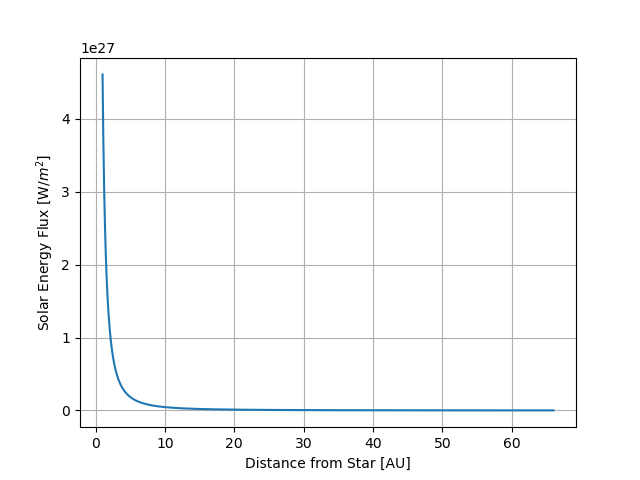
\includegraphics[scale=0.4]{Figures/Radius_flux}
		\caption{The electromagnetic flux as a function of distance from the star in our solar system.}\label{fig:Radius_Flux}
	\end{figure}

	\begin{table}[h]
	    \begin{tabular}{|c|c|c|c|c|}
	        %% l (Left aligned), c (Centered), r (Right aligned)
	        \hline
			Planet 0 & Planet 1 & Planet 2 & Planet 3\\
	        \hline
			2375 & 1765 & 560.9 & 48.86\\
			\hline\hline
			Planet 4 & Planet 5 & Planet 6 & Planet 7\\
	        \hline
			130.1 & 284.0 & 76.74 & 5140\\
			\hline
	    \end{tabular}
	    \caption{Electromagnetic flux at each planets surface when it is at the semi-major axis of it's orbit. All values are in W/$m^2$.}
	    \label{tab:planet_flux}
	\end{table}

	We can clearly see a correspondence between the radius from the star increasing and the flux decreasing.
	The flux is decreasing rapidly until approximately 4 AU, and is then flattening and decreasing a lot less at a distance greater than approximately 8 AU.
	The amount of radiation will therefore be quite high for the inner planets and a lot less and relatively equal for the outer planets.




\subsection{Temperature}\label{subsec:temperature-results}
	Based on the flux and formula~\eqref{Planet_temp}, the temperature was calculated as described in the previous section.
	Figure~\ref{fig:Radius_Temp} visualizes the temperature as a function of the distance from the star in our solar system.

	\begin{figure}[h]
		%% H(Here), h(here approx), t(top of page), b(bottom of page)
		\centering
		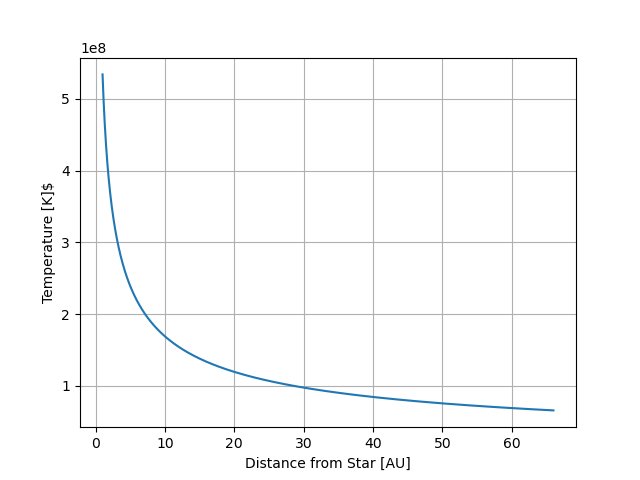
\includegraphics[scale=0.4]{Figures/Radius_temp}
		\caption{The temperature of a black body as a function of the distance between the body and the star.}\label{fig:Radius_Temp}
	\end{figure}

	Just like the flux, the temperature is most interesting at the surface of the planets.
	Therefore, the temperature on the surface of each planet has been calculated using formula~\eqref{Planet_temp} and the method described in section~\ref{sec:method} .

	\begin{table}[h]
			\begin{tabular}{|c|c|c|c|c|}
				%% l (Left aligned), c (Centered), r (Right aligned)
				\hline
				Planet 0 & Planet 1 & Planet 2 & Planet 3\\
				\hline
				452.4 & 420.0 & 315.4 & 171.3\\
				\hline\hline
				Planet 4 & Planet 5 & Planet 6 & Planet 7\\
				\hline
				218.8 & 266.0 & 191.8 & 548.7\\
				\hline
			\end{tabular}
			\caption{Temperature at each planets surface when it is at the semi-major axis of it's orbit. All values are in degrees Kelvin.}
			\label{tab:planet_temp}
		\end{table}

	The graph in figure~\ref{fig:Radius_Temp} shows the temperature decreasing as the radius decreases.
	The same applies for the calculated values for the surface temperature of the planets.
	The temperatures range between $171.3^{\circ}$ K on the surface of planet 3 and $548.7^{\circ}$ K on the surface of planet 7 with semi-major axes of respectively $65.6343$ AU and $6.16055$ AU
	As seen in Figure~\ref{fig:Radius_Temp} the temperature decreases similarly to the flux.
	However, the temperature does not decrease as rapidly in the innermost part of the solar system and has a smoother transition to the temperature gradient in the outer part of the solar system.\\


\subsection{The Habitable zone}\label{subsec:the-habitable-zone-results}
	The habitable zone has been defined as the zone around the star where the temperature on a planet is between $260$ and $390$ degrees Kelvin.
	Using formula~\eqref{Radius_temp}, which is a rearrangement of formula~\eqref{Planet_temp}, the inner and outer boundaries of the habitable zone can be determined.
	The inner boundary is found to be $12.532$ AU and the outer boundary is found to be $28.197$ AU.
	All planets at a distance greater than the inner boundary and less than the outer boundary lie within the habitable zone of our solar system.
	This includes Planet 2 and Planet 5\\

	To design our rover, we were also trying to find the correct size of solar panels.
	This was calculated based on the flux reaching the solar panels of the rover at a given distance, the efficiency of the solar panels and the required power for the rover.
	The rover requires 40 Watts of electric power to keep its electric systems running.
	It can be seen in figure~\ref{fig:Radius_area} that is increasing as the distance to the star increases.
	This means if the rover is going further out in the solar system, it needs to be equipped with larger solar panels to provide enough power.
	This makes sense as the flux, and therefore power reaching the solar panels per square meter decreases with increasing distance.
	The size of the solar panels therefore needs to increase to capture the same amount of solar power.

	\begin{figure}[h]
		%% H(Here), h(here approx), t(top of page), b(bottom of page)
		\centering
		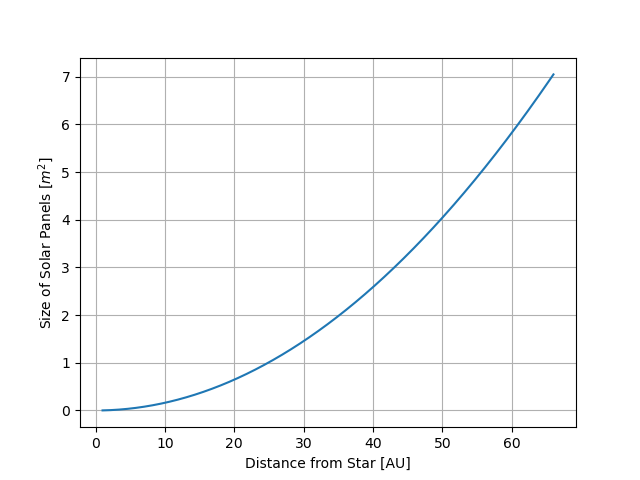
\includegraphics[scale=0.4]{Figures/Radius_area}
		\caption{The required area of the solar panels on the rover to provide 40 W with 12\% efficiency.}\label{fig:Radius_area}
	\end{figure}

	As we will be going to land on a planet, we need to know the required size when we are on a planet.
	Therefore, the required solar panel size has been calculated for each planet and is listed in table~\ref{tab:panel_sizes}.

	\begin{table}[h]
			\begin{tabular}{|c|c|c|c|c|}
				%% l (Left aligned), c (Centered), r (Right aligned)
				\hline
				Planet 0 & Planet 1 & Planet 2 & Planet 3\\
				\hline
				0.140 & 0.189 & 0.594 & 6.823\\
				\hline\hline
				Planet 4 & Planet 5 & Planet 6 & Planet 7\\
				\hline
				2.563 & 1.174 & 4.344 & 0.065\\
				\hline
			\end{tabular}
			\caption{Solar panel size required when the rover is on each planets surface when they are on their semi-major axis of their orbits. All values are in $m^2$.}
			\label{tab:panel_sizes}
		\end{table}

	The most suitable planet for our mission seems to be Planet 5.
	This planet is a rock planet with a semi-major axis of 27.7773 AU.
	It's temperature is $266.0^{\circ}$ K or $-7.13^{\circ}$ C, which means it lies within the habitable zone.\\


\subsection{Gravitational forces}\label{subsec:gravitational-forces}
	To perform an orbit injection maneuver into the orbit of Planet 5 we want to find the distance from the planet at which the gravitational force from the planet is a certain amount larger than the gravitational force from the star.
	In figure the ratio $k$ between the gravitational force form the planet and star is graphed as a function of the distance from the planet.

	\begin{figure}[h]
		%% H(Here), h(here approx), t(top of page), b(bottom of page)
		\centering
		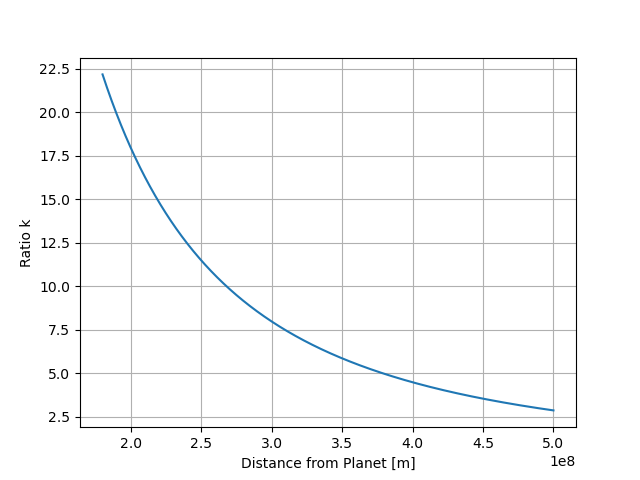
\includegraphics[scale=0.4]{Figures/Grav_ratio_k}
		\caption{The ratio between the gravitational force from the planet and star as a function of the distance from the planet.}\label{fig:k_ratio_dist}
	\end{figure}

	The ratio is decreasing with the distance increasing.
	This means if we want to start the injection maneuver at a position with a higher k-value to make it easier, we need to decrease the distance to the planet.


\subsection{Image of the Planet}\label{subsec:image-of-the-planet}
	Our rover is equipped with a camera with a 35 mm full format image sensor and a lens with a focal length of 800 mm.
	The field of view is therefore approximately 2.6 degrees.
	Using these specifications as well as the radius of Planet 5, formula~\eqref{Image_Dist} has been used to determine the maximum distance for a resolved image of the Planet 5.
	To get an overview over the necessary resolution fo the camera, the required number of pixels in the image sensor in one dimension has been graphed as a function of the distance in figure~\ref{fig:Res_pixels}.

	\begin{figure}[h]
		%% H(Here), h(here approx), t(top of page), b(bottom of page)
		\centering
		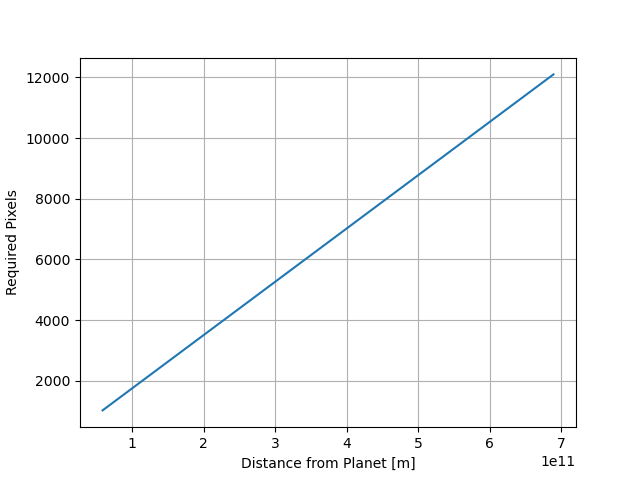
\includegraphics[scale=0.4]{Figures/Res_pixels}
		\caption{The necessary number of pixels in the image sensor in one dimension as function of the distance from the planet.}\label{fig:Res_pixels}
	\end{figure}

	In figure~\ref{fig:Res_pixels} it can be seen that the number of required pixels in one dimension of the image sensor is linearly dependent of the maximum distance.
	This means the better the resolution of the camera, the further away the image of the planet will appear resolved.
	Furthermore, the narrower the field of view, the further away the planet will appear resolved on an image.


\section{Discussion} \label{sec:discussion}
	\subsection{Electromagnetic Radiation}\label{subsec:disc_radiation}
	According to our results~\ref{fig:Radius_Flux}, the electromagnetic flux is decreasing very rapidly with increasing distance to the star during the first 4 AU.
	Between approximately 4 and 8 AU, the rate at which the flux decreases, levels out.
	Further out than 8 AU, the decrease of electromagnetic flux is relatively low compared to closer to the star.\\
	The flux decreasing this way makes a lot of sense, since it is inversely proportional with the square of the distance to the sun according to equation~\eqref{Flux_Distance}.
	However, the difference of the rate of decrease is still surprising, when comparing a point very close to the star and very far away from the star.

	Since our rover only requires 40 Watts of power to keep its electrical instruments and communication running, the solar array can be between $0.065$ m$^2$ at planet 7 and $6.823$ m$^2$ at planet 3.
	At planet 5, the panel size is $1.174$ m$^2$, which is a relatively small size for a rover.
	This will be a big advantage, as we can make the rover, and therefore the rocket more compact.\\
	Something we decided to neglect, is the possibility of a planet coming in the way between the star and our spacecraft or rover.
	This would result in the electromagnetic radiation being blocked from reaching the rover.\\
	However, since there is so much space between the planets, the probability of this happening are quite small.
	Furthermore, the rover can temporarily be put in an energy-saving state, if such an event should happen.\\

\subsection{Temperature and habitable zone}\label{subsec:disc_temperature}
	When looking at the results of the temperature~\ref{fig:Radius_Temp}, we see that the temperature is decreasing.
	However, the change of rate of decrease is smoother compared to the flux.\\
	When looking at the temperatures~\ref{tab:planet_temp}, we see that only planet 2 and 5 are within the habitable zone.
	This makes sense as the orbits of those two planets are close to each other, as well as not being far on the inside or outside of the solar system.\\
	A temperature of $266^{\circ}$ Kelvin, or $-7.15^{\circ}$ Celsius, means that liquid water can exist.\\
	Note that these temperatures are at the aphelion.
	This means, the planet will be at this distance or closer to the sun, which means the temperature will often be a bit higher than the value we found.\\
	Furthermore, we have to note that the temperature will depend on the day-night-cycle.
	The side facing towards the star will be a lot warmer than the side facing away from the star.

\subsection{Gravitational forces}\label{subsec:disc_gravitational-forces}
	We see that the ratio of the gravitational forces from the star and planet varies greatly at close distances to the planet.
	Since the gravitational force is inversely proportional to the square of the distance between the objects, we will not see a lot of difference in the forces from the star when being close to the planet.
	Even with such a large mass as the star.
	However, as we are close to the planet, its gravitational force will vary a lot.
	Therefore, the ratio of the forces varies a lot when the spacecraft is close to the planet and a lot less when being further away.
	When performing an injection maneuver, we want a ratio of $k = 10$, which means we have to be at a distance of $268'000$ km from the planet.
	This sound reasonable for an orbit around a planet.

\subsection{Imaging the planet}\label{subsec:disc_imaging-the-planet}
	When looking at the results the requirements of taking a resolved picture, we see a linear relationship between the maximum distance and the number of pixels in one dimension of the sensor.
	Since the sensor is a square, the total number of required pixels will be proportional to the square of the distance.\\
	However, a higher resolution is not necessarily better, as it often means higher costs and larger, more sensitive equipment.
	Therefore, we will first have to simulate our trajectory to determine how close we can approach the planet before we need a picture to orient ourselves.

\section{Conclusion} \label{sec:conclusion}
	In this paper, an expression for the electromagnetic flux based on the distance from the star in our solar system has been successfully determined.
	Furthermore, a connection between the flux and the temperature of a planet at a given distance has been deduced, and determined.\\
	Using the expression for the temperature, the boundaries of the habitable zone have been determined, and which planets lie in said zone.
	In our case, the planets inside this zone are planet 2 and 5.
	The results we have received agree quite well with our expectations.\\
	Since we want to land a rover on our destination planet, we used the expression for the flux to determine the required size of the solar panels of the rover.
	This lead to a very reasonable result.\\
	However, before landing the rover, our spacecraft first needs to reach the planet and enter orbit around it.
	To do this we have found an expression, which relates the gravitational forces of the star on the spacecraft to the gravitational forces of the planet on the spacecraft.
	This expression has been used to find the required distance from the planet to achieve a certain ratio between the forces.\\
	Additionally, a relationship between the maximum distance at which the spacecraft is able to take a resolved picture and the camera resolution has been determined.
	These results will be extremely useful in further planning and simulations of our mission of sending the spacecraft to our destination.

\section{Appendix: Mathematical Derivations}
	\subsection{The habitable zone}\label{subsec:app-the-habitable-zone}
	Using~\eqref{stefan_boltzmann_law} and~\eqref{Flux_Distance} we find
	\begin{align}
		&T_{Planet} = \sqrt[4]{\frac{F}{\sigma}}\\
		&T_{Planet} = \sqrt[4]{\frac{R_{Star}^2 T_{Star}^4}{r^2}} \label{Planet_temp}
	\end{align}
	\begin{align}
		&r^2 = \frac{R_{Star}^2 T_{Star}^4}{T_{Planet}^4}\\
		&r = \frac{R_{Star} T_{Star}^2}{T_{Planet}^2}
	\end{align}


	\subsection{Gravitational forces}\label{subsec:app-gravitational-forces}
    By inserting equations~\eqref{G_Planet} and~\eqref{G_Star} into equation~\eqref{grav_forces}, we find
	\begin{align*}
    	\gamma \, \frac{M_{SC}M_{Planet}}{l^2} &= k\, \gamma \, \frac{M_{SC}M_{Star}}{|\textbf{r}|^2}\\
		\frac{M_{Planet}}{l^2} &= k\, \frac{M_{Star}}{|\textbf{r}|^2}\\
		l^2 =& \frac{M_{Planet}|\textbf{r}|^2}{k\,M_{Star}}\\
		l =& |\textbf{r}|\sqrt{\frac{M_{Planet}}{k\,M_{Star}}}
	\end{align*}\\


\newpage
\printbibliography



\end{document}